\subsection{Fase di validazione e collaudo}

\subsubsection{Completamento dell'implementazione e raffinamento delle funzionalità}

\paragraph{Incremento VIII}\mbox{}\\
I dati riportati di seguito si riferiscono al periodo che va dal 09-04-2021 al 16-04-2021.

\begin{minipage}[b]{0.65\linewidth}
\begin{small}

\begin{longtable}{ c | c c c c c c | c} 
 \rowcolor{coloreRosso}
 \color{white}{\textbf{Nominativo}} &
 \color{white}{\textbf{RE}} &
 \color{white}{\textbf{AM}} &
 \color{white}{\textbf{AN}} &
 \color{white}{\textbf{PT}} &
 \color{white}{\textbf{PR}} &
 \color{white}{\textbf{VE}} &
 \color{white}{\textbf{Tot.}} \\
 	
 \BM{} & - & 3 & - & - & - & 4 & 7 \\ 
 \PA{} & 1 & 2 & - & 3 & - & - & 6 \\ 
 \RA{} & 4 & - & - & - & - & 2 & 6 \\ 
 \SH{} & - & - & - & 5 & 1 & - & 6 \\ 
 \SG{} & - & - & - & - & 4 & 2 & 6 \\ 
 \SP{} & - & - & - & 4 & - & 3 & 7 \\ 
 \ZM{} & - & 2 & - & - & 2 & 2 & 6 \\
 
 	\rowcolor{coloreRosso}
 	\color{white}{\textbf{Totale ore ruolo}} &
 	\color{white}{\textbf{5}} &
 	\color{white}{\textbf{7}} &
 	\color{white}{\textbf{-}} &
 	\color{white}{\textbf{12}} &
 	\color{white}{\textbf{7}} &
 	\color{white}{\textbf{13}} &
 	\color{white}{\textbf{44}} \\
	\rowcolor{white}
	\captionsetup{width=.9\textwidth}
 	\caption{Distribuzione delle ore nell'incremento VIII}
\end{longtable}

\end{small}
\end{minipage}
\begin{minipage}[b]{.3\linewidth}
\begin{small}

\begin{longtable}{ c | c | c} 
 	\rowcolor{coloreRosso}
 	\color{white}{\textbf{Ruolo}} &
 	\color{white}{\textbf{Ore}} &
 	\color{white}{\textbf{Costo €}} \\
 	
 	Responsabile & 5 & 150\\
 	Amministratore & 7 & 140\\
 	Analista & - & -\\
 	Progettista & 12 & 264\\
 	Programmatore & 7 & 105\\
 	Verificatore & 13 & 195\\
 	
 	\rowcolor{coloreRosso}
 	\color{white}{\textbf{Totale}} &
 	\color{white}{\textbf{44}} &
 	\color{white}{\textbf{854 €}}\\
 	\rowcolor{white}
 	\caption{Costi per ruolo nell'incremento VIII}
\end{longtable}

\end{small}
\end{minipage}

\begin{figure}[!htb]   
    \centering
    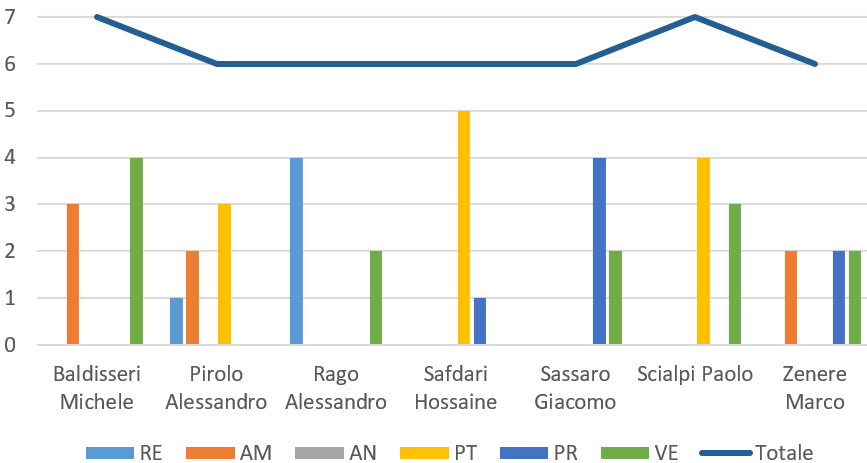
\includegraphics[width=0.90\textwidth]{Images/prev8}
	\caption{Ripartizione oraria per ciascun membro nell'incremento VIII}
\end{figure}

\paragraph{Incremento IX}\mbox{}\\
I dati riportati di seguito si riferiscono al periodo che va dal 16-04-2021 al 23-04-2021.

\begin{minipage}[b]{0.65\linewidth}
\begin{small}

\begin{longtable}{ c | c c c c c c | c} 
 \rowcolor{coloreRosso}
 \color{white}{\textbf{Nominativo}} &
 \color{white}{\textbf{RE}} &
 \color{white}{\textbf{AM}} &
 \color{white}{\textbf{AN}} &
 \color{white}{\textbf{PT}} &
 \color{white}{\textbf{PR}} &
 \color{white}{\textbf{VE}} &
 \color{white}{\textbf{Tot.}} \\
 	
 \BM{} & - & 2 & - & - & 4 & 1 & 7 \\ 
 \PA{} & 3 & - & - & 3 & 2 & - & 8 \\ 
 \RA{} & 3 & - & - & - & - & 3 & 6 \\ 
 \SH{} & - & 3 & - & - & 2 & 3 & 8 \\ 
 \SG{} & - & - & - & - & 3 & 4 & 7 \\ 
 \SP{} & 2 & - & - & - & - & 5 & 7 \\ 
 \ZM{} & - & 2 & - & - & 2 & 4 & 8 \\
 
 	\rowcolor{coloreRosso}
 	\color{white}{\textbf{Totale ore ruolo}} &
 	\color{white}{\textbf{8}} &
 	\color{white}{\textbf{7}} &
 	\color{white}{\textbf{-}} &
 	\color{white}{\textbf{3}} &
 	\color{white}{\textbf{13}} &
 	\color{white}{\textbf{20}} &
 	\color{white}{\textbf{51}} \\
	\rowcolor{white}
	\captionsetup{width=.9\textwidth}
 	\caption{Distribuzione delle ore nell'incremento IX}
\end{longtable}

\end{small}
\end{minipage}
\begin{minipage}[b]{.3\linewidth}
\begin{small}

\begin{longtable}{ c | c | c} 
 	\rowcolor{coloreRosso}
 	\color{white}{\textbf{Ruolo}} &
 	\color{white}{\textbf{Ore}} &
 	\color{white}{\textbf{Costo €}} \\
 	
 	Responsabile & 8 & 240\\
 	Amministratore & 7 & 140\\
 	Analista & - & -\\
 	Progettista & 3 & 66\\
 	Programmatore & 13 & 195\\
 	Verificatore & 20 & 300\\
 	
 	\rowcolor{coloreRosso}
 	\color{white}{\textbf{Totale}} &
 	\color{white}{\textbf{51}} &
 	\color{white}{\textbf{941 €}}\\
 	\rowcolor{white}
 	\caption{Costi per ruolo nell'incremento IX}
\end{longtable}

\end{small}
\end{minipage}

\begin{figure}[!htb]   
    \centering
    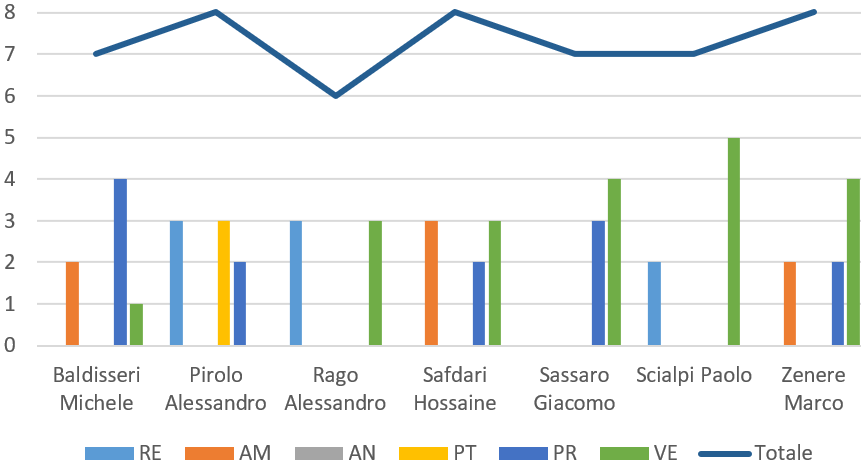
\includegraphics[width=0.95\textwidth]{Images/prev9}
	\caption{Ripartizione oraria per ciascun membro nell'incremento IX}
\end{figure}

\subsubsection{Verifica e collaudo}

I dati riportati di seguito si riferiscono al periodo che va dal 23-04-2021 al 03-05-2021.

\begin{minipage}[b]{0.65\linewidth}
\begin{small}

\begin{longtable}{ c | c c c c c c | c} 
 \rowcolor{coloreRosso}
 \color{white}{\textbf{Nominativo}} &
 \color{white}{\textbf{RE}} &
 \color{white}{\textbf{AM}} &
 \color{white}{\textbf{AN}} &
 \color{white}{\textbf{PT}} &
 \color{white}{\textbf{PR}} &
 \color{white}{\textbf{VE}} &
 \color{white}{\textbf{Tot.}} \\
 	
 \BM{} & - & - & - & - & - & 6 & 6 \\ 
 \PA{} & 2 & 2 & - & - & 2 & - & 6 \\ 
 \RA{} & 3 & 4 & - & - & - & 1 & 8 \\ 
 \SH{} & - & - & - & - & 4 & 2 & 6 \\ 
 \SG{} & - & - & - & - & 2 & 5 & 7 \\ 
 \SP{} & 2 & - & - & - & - & 4 & 6 \\ 
 \ZM{} & - & - & - & - & 2 & 4 & 6 \\

 	\rowcolor{coloreRosso}
 	\color{white}{\textbf{Totale ore ruolo}} &
 	\color{white}{\textbf{7}} &
 	\color{white}{\textbf{6}} &
 	\color{white}{\textbf{-}} &
 	\color{white}{\textbf{-}} &
 	\color{white}{\textbf{10}} &
 	\color{white}{\textbf{22}} &
 	\color{white}{\textbf{45}} \\
	\rowcolor{white}
	\captionsetup{width=.9\textwidth}
 	\caption{Distribuzione delle ore nel periodo III della Progettazione architetturale}
\end{longtable}

\end{small}
\end{minipage}
\begin{minipage}[b]{.3\linewidth}
\begin{small}

\begin{longtable}{ c | c | c} 
 	\rowcolor{coloreRosso}
 	\color{white}{\textbf{Ruolo}} &
 	\color{white}{\textbf{Ore}} &
 	\color{white}{\textbf{Costo €}} \\
 	
 	Responsabile & 7 & 210\\
 	Amministratore & 6 & 120\\
 	Analista & - & -\\
 	Progettista & - & -\\
 	Programmatore & 10 & 150\\
 	Verificatore & 22 & 330\\
 	
 	\rowcolor{coloreRosso}
 	\color{white}{\textbf{Totale}} &
 	\color{white}{\textbf{65}} &
 	\color{white}{\textbf{810 €}}\\
 	\rowcolor{white}
 	\caption{Costi per ruolo nel periodo III della Progettazione architetturale}
\end{longtable}

\end{small}
\end{minipage}

\begin{figure}[!htb]   
    \centering
    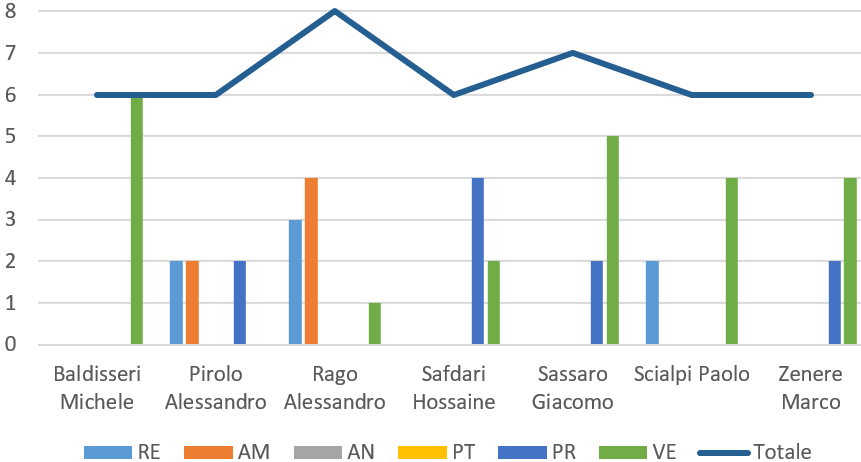
\includegraphics[width=0.95\textwidth]{Images/prev10}
	\caption{Ripartizione oraria per ciascun membro durante l'incremento X}
\end{figure}

\subsubsection{Riepilogo}

\begin{minipage}[b]{0.65\linewidth}
\begin{small}

\begin{longtable}{ c | c c c c c c | c} 
 \rowcolor{coloreRosso}
 \color{white}{\textbf{Nominativo}} &
 \color{white}{\textbf{RE}} &
 \color{white}{\textbf{AM}} &
 \color{white}{\textbf{AN}} &
 \color{white}{\textbf{PT}} &
 \color{white}{\textbf{PR}} &
 \color{white}{\textbf{VE}} &
 \color{white}{\textbf{Tot.}} \\
 	
 \BM{} & - & 5 & - & - & 4 & 11 & 20 \\ 
 \SG{} & - & - & - & - & 9 & 11 & 20 \\ 
 \SH{} & - & 3 & - & 5 & 7 & 5 & 20 \\ 
 \PA{} & 6 & 4 & - & 6 & 4 & - & 20 \\ 
 \SP{} & 4 & - & - & 4 & - & 12 & 20 \\ 
 \RA{} & 10 & 4 & - & - & - & 6 & 20 \\ 
 \ZM{} & - & 4 & - & - & 6 & 10 & 20 \\
 
 \rowcolor{coloreRosso}
 	\color{white}{\textbf{Totale ore ruolo}} &
 	\color{white}{\textbf{20}} &
 	\color{white}{\textbf{20}} &
 	\color{white}{\textbf{-}} &
 	\color{white}{\textbf{15}} &
 	\color{white}{\textbf{30}} &
 	\color{white}{\textbf{55}} &
 	\color{white}{\textbf{140}} \\
 	\rowcolor{white}
 	\captionsetup{width=.9\textwidth}
 	\caption{Distribuzione delle ore nel periodo di Validazione e Collaudo}
\end{longtable}
\end{small}
\end{minipage}
\begin{minipage}[b]{.3\linewidth}
\begin{small}

\begin{longtable}{ c | c | c} 
 	\rowcolor{coloreRosso}
 	\color{white}{\textbf{Ruolo}} &
 	\color{white}{\textbf{Ore}} &
 	\color{white}{\textbf{Costo €}} \\
 	
 	Responsabile & 20 & 600\\
 	Amministratore & 20 & 400\\
 	Analista & - & -\\
 	Progettista & 15 & 330\\
 	Programmatore & 30 & 450\\
 	Verificatore & 55 & 825\\
 	
 	\rowcolor{coloreRosso}
 	\color{white}{\textbf{Totale}} &
 	\color{white}{\textbf{350}} &
 	\color{white}{\textbf{2605 €}}\\
 	\rowcolor{white}
 	\caption{Costi per ruolo nel periodo di Validazione e Collaudo}
\end{longtable}

\end{small}
\end{minipage}

I seguenti grafici riassumo i dati ottenuti.

\begin{figure}[!htb]
   \begin{minipage}{0.6\textwidth}
     \centering
     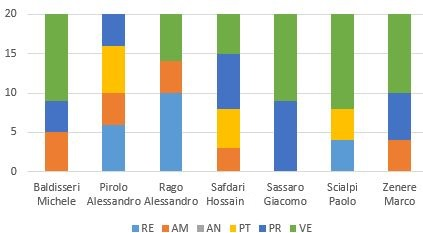
\includegraphics{Images/PO-Verifica}
     \caption{Ripartizione oraria per ciascun membro nella fase di Validazione e Collaudo}
   \end{minipage}\hspace{0.1\textwidth}
   \begin{minipage}{0.3\textwidth}
     \centering
     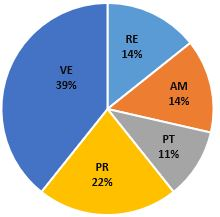
\includegraphics[width=.9\textwidth]{Images/PE-Verifica}
     \captionsetup{width=1\textwidth}
     \caption{Ripartizione ore totali nella fase di Validazione e Collaudo}
   \end{minipage}
\end{figure}